\documentclass[]{elsarticle}

\usepackage[T1]{fontenc}
\usepackage{multicol}
\usepackage{tabularx}
%\usepackage{tabulary}
\usepackage{graphicx}
\usepackage[margin=0.8in]{geometry}
\usepackage{color}
\PassOptionsToPackage{hyphens}{url}\usepackage{hyperref}
\usepackage[usenames,dvipsnames,svgnames,table]{xcolor}
\hypersetup{colorlinks=true, citecolor=blue}

\usepackage{tocloft}
\usepackage{float}
\usepackage{mathtools}
\DeclarePairedDelimiter\ceil{\lceil}{\rceil}
\DeclarePairedDelimiter\floor{\lfloor}{\rfloor}

%\linespread{3}
%\usepackage{lineno}
%\linenumbers

\makeatletter
\def\ps@pprintTitle{%
	\let\@oddhead\@empty
	\let\@evenhead\@empty
	\let\@oddfoot\@empty
	\let\@evenfoot\@oddfoot
}
\makeatother

%opening

\begin{document}
	
	\onecolumn
	
	\begin{abstract}
		\par The potential of multi-spectral images is growing rapidly in precision agriculture,
		and is currently based on the use of multi-sensor cameras. However, their development usually concerns aerial application and their parameters are optimized to high altitudes per drone ($\approx 50$ meters)
		to ensure surface coverage and reduce technical problems.
		%As part of the efforts towards of phytosanitary use reduction,
		%this type of device becomes necessary in order to discriminate crops from weeds in close detection ($< 10$ meters).
		%Maximize specific trait extraction (spectral index, shape, texture, \dots) requires high spatial resolution to allow precise weed classification.
		With the recent emergence of terrestrial robots (UGV), their use is diverted for nearby agronomic applications.
		It is possible to explore new application maximizing specific traits extraction (spectral index, shape, texture \dots) which requires high spatial resolution
		\\
		\par The problem with these cameras is that all sensors are not aligned and the manufacturers' methods are not adapted for close-field acquisition,
		resulting in offsets between images and degrading the quality of extractable information.
		We therefore need a solution to align the different images accurately in such condition.
		The objective of this article is to propose a simple method that allows to define the ideal conditions
		for matching multi-spectral images from the multi-sensor camera at low heights of use applied on agronomic scenes.
		\\
		\par In this study we propose a two-step method applied to the six-bands Airphen multi-sensors camera with
		(i) affine correction using pre-calibrated matrix at different heights, the closest transformation can be selected via internal GPS
		and (ii) perspective correction to refine the previous one, using key-points matching between enhanced gradients of each spectral bands.
		Nine types of key-point detection algorithms (ORB, GFTT, AGAST, FAST, AKAZE, KAZE, BRISK, SURF, MSER) with three different modalities of parameters
		was evaluated for their benchmark and their corresponding best reference spectra.
	\end{abstract}
	
	\begin{keyword}
		Registration \sep
		Multi-spectral imagery \sep
		Precision farming \sep
		Feature descriptor
	\end{keyword}
	
	\begin{frontmatter}
		\title{Two-step multi-spectral registration \\ via key-point detector and gradient similarity}
		\author[unilu]{Jehan-Antoine VAYSSADE} \ead{jehan-antoine.vayssade@inra.fr}
		\author[unilu]{Christelle Gee} \ead{christelle.gee@agrosupdijon.fr}
		\address[myuni]{Agroécologie, AgroSup Dijon, INRA, Univ. Bourgogne, Univ. Bourgogne Franche-Comté, F-21000 Dijon, France}
		\date{Received: date / Accepted: date}
	\end{frontmatter}
	
	\newpage
	
	\section{Introduction}
	
	\par Modern agriculture is changing towards a system that is less dependent on pesticides \cite{10.1371/journal.pone.0097922}
	(herbicides remain the most difficult pesticides to reduce) and digital tools are of great help in his matter.
	The development of imaging and image processing have made it possible to characterize an agricultural plot \cite{SANKARAN2015112}
	(crop health status or soil characteristics) using non-destructive agronomic indices \cite{doi:10.1080/02757259509532298, filella1995evaluating, 10.1371/journal.pone.0072736}
%	(NDVI \footnote{Normalized Difference Vegetation Index}, ExcessGreen, \dots)
	replacing traditional destructive and time-consuming methods.
	In recent years, the arrival of miniaturized multi-spectral and hyper-spectral cameras on Unmanned Aerial Vehicles (UAVs)
	has allowed the plot spatio-temporal monitoring of the field. These vision systems have been developed for precise working conditions (flight height $50m$).
	Although, very practical to use, they are also used for proxy-sensing applications.
	However, the algorithms for correcting and matching multiple single-band images of different spectral range,
	offered by manufacturers, are not optimal for low heights. It thus requires a specific close-field image registration.
	% To do so, an image registration is necessary.
	\\
	\par Image registration is the process of transforming different images of one scene into the same coordinate system.
	The spatial relationships between these images can be rigid (translations and rotations), affine (shears for example),
	homographic, or complex large deformation models (due to the difference of depth between ground and leafs) \cite{Kamoun}.
	The main difficulty is that multispectral cameras have low spectral coverage between bands, resulting in a loss of characteristics between them.
	Which is caused by (i) plant leaves have a different aspect depending on the spectral bands
	(ii) there are highly complex and self-similar structures in our images \cite{douarre:hal-02183837}.
	It therefore affects the process of detecting common characteristics between bands for image registration.
	%(iii) and the scene are a grassland or agriculture image at different scale,
	%which is a complex spectral scene making a hard fit for such a registration.
	There is two types of registration, feature based and intensity based \cite{Zitova}.
	(i) Feature based methods by extract point of interest and using feature matching, in most cases a brute-force matching is used, making those techniques slow.
	Fortunately these features can be filtered to reduce the matching cost depending of the spatial properties we have, and a GPGPU implementation can reduce the comparisons cost.
	(ii) Intensity-based automatic image registration is an iterative process, and the metrics used are sensitive to determine the numbers of iteration,
	making such method computationally expensive for precise registration. Furthermore multi-spectral need different metrics for each registered bands which is hard to achieve.
	\\
	\par Different studies of images alignment using multi-sensors camera can be found for acquisition using UAV at medium and high distance.
	Some show good performances (in term of number of key-points) for feature based \cite{DantasDiasJunior, Vakalopoulou} with strong enhancement of feature descriptor for matching performances.
	Other do not and prefer to use intensity based \cite{douarre:hal-02183837} on better convergence metrics \cite{8118101} (in term of correlation),
	which is slower and not necessarily robust against light variability \cite{Vioix2004ConceptionER}.
	And their optimization can also fall into a local minimum.
	\\
	\par Traditional approach to multi-spectral image recording is to designate one channel as the target channel and record all the others on the selected one.
	Currently, only \cite{DantasDiasJunior} show a methods for selecting the best reference, but there is no studies who as defined the best spectral reference in agronomic scene.
	In all cases NIR (850nm) or the middle range spectral reference are conventionally used without studying the others on precision agriculture.
	In addition those studies mainly propose features matching without large methods comparison \cite{DantasDiasJunior}(less than 4) of their performance (time/precision),
	without showing the importance of the spectral reference and the normalized gradients transformation like in Intensity-based methods.
	%spectral band reference selection, or pre-affine correction depending on the distance.
	\\
	\par However, despite the growing use of UGVs and multi-spectal imaging, the domain is not very well sourced,
	and no studies have been found under agricultural and external conditions in near field of view (less than 10 meter) for multi-spectral registration.
	Thus, this study propose a benchmark of popular feature extractor inside normalized gradients transformation and the best spectral reference was defined for each of them.
	Moreover a pre-affine registration is used to filter the feature matching, evaluated at different spatial resolution.
	So this study shows the importance of the selection of the reference and the features extractor on normalized gradients in such registration.
	%\\
	%\par In this study we have preferred not to enhance features by the information send to each features methods,
	%as example SIFT have been rejected on the paper \cite{douarre:hal-02183837}
	%which explain that the matched features are two numerous and not greatly matched.
	
	\newpage
	\section{Material and Method}
	
	\subsection{Material}
	
	The multi-spectral imagery is provided by the six-band multi-spectral camera Airphen \footnote{\url{https://www.hiphen-plant.com/our-solutions/airphen/}}.
	AIRPHEN is a scientific multi-spectral camera developed by agronomists for agricultural applications.
	It can be embedded in different types of platforms such as UAV, phenotyping robots, etc.
	\\
	\par AIRPHEN is highly configurable (bands, fields of view), lightweight and compact.
	It can be operated wirelessly and combined with complementary thermal infrared channel and high resolution RGB cameras.
	The camera was configured using 450/570/675/710/730/850 nm with FWHM \footnote{Full Width at Half Maximum} of 10nm, the position of each bands is referenced on table \ref{tab:bands-disposition}.
	The focal lens is 8mm. The raw resolution for each spectral band is $1280x960$ px with 12 bit of precision.
	Finally the camera also provides an internal GPS antenna, that can be used to get the distance from the ground.
	
	\begin{table}[H]
		\begin{tabularx}{\linewidth}{|X|X|X|}
			\hline
			450 & 675 & 710 \\
			\hline
			570 & 850 & 730 \\
			\hline
		\end{tabularx}
		\label{tab:bands-disposition}
		\caption{Disposition of each bands on the Airphen multi-sensors camera}
	\end{table}
	
	\par Two datasets were taken at different heights with images of a chessboard and of an agronomic scene.
	We have used a metallic gantry for positioning the camera at different heights.
	The size of the gantry is $3m * 5m * 4m$.
	Due to the size of the chessboard, the limited focus of the camera and the gantry height,
	we have bounded the acquisition height from $1.6m$ to $5m$ with $20cm$ steeps, which represent 18 acquisitions.
	\\
	\par The first dataset is for the calibration. A chessboard is taken at different heights, the corresponding data can be found in \textit{data/step-chess/}.
	The second one is for the alignment verification under real conditions.
	One shot of an agronomic scene is taken at different heights, the corresponding data can be found in \textit{data/step/}
	with a bias of $\pm 10cm$ to be in the worst case (most complex).
	
	\subsection{Methods}
	
	Alignment is refined in two stages, with (i) affine registration approximately estimated
	and (ii) perspective registration for the refinement and precision.
	As example the figure \ref{fig:each-stages} shows each correction step, where the first line is for the (i) affine correction (section \ref{sec:affine}), the second and third is for (ii) perspective correction.
	More precisely the second are per-channel pre-processing where feature detectors are used to detect key points (section \ref{sec:pre-processing}).
	And the last line each channel key points are associated to compute the perspective correction through homography, to the selected spectral band (section \ref{sec:perspective}).
	Those steps are explained on specific subsections.
	
	\begin{figure}[H]
		\centering
		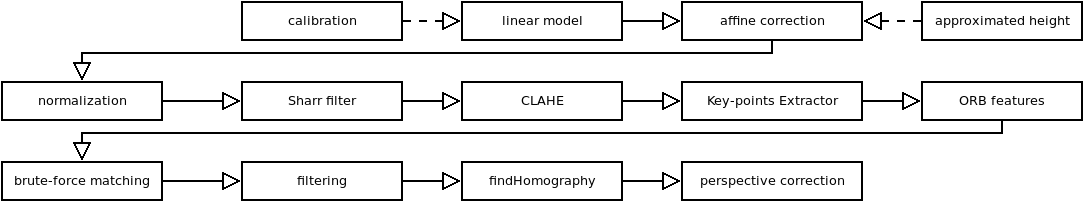
\includegraphics[width=\linewidth]{../figures/step.png}
		\caption{Each stages}
		\label{fig:each-stages}
	\end{figure}

	%As example the figure \ref{fig:merged-correction} show each correction steep at 1.6 meters.
	%
	%\begin{figure}[!htb]
	%	\centering
	%	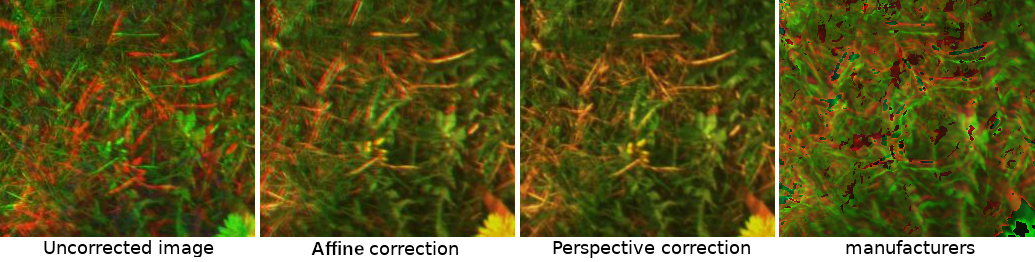
\includegraphics[width=\linewidth]{../figures/merged-correction.png}
	%	\caption{Exemple of each correction}
	%	\label{fig:merged-correction}
	%\end{figure}
	
	\subsubsection{Affine Correction}
	\label{sec:affine}
	
	It is important to notice the closer we take the snapshot, the bigger is the distance of the initial Affine Correction.
	On the other hand at a distance superior or equals to $5m$, the initial affine correction become stable (figure \ref{fig:affine-translation-height}).
	Then a calibration is used to build a linear model, which makes the affine correction to work at any height.
	The main purpose of this step is to reduce the offset between each spectral band,
	which allows the similarity to be spatially delimited within a few pixels, making feature matching more effective.
	
	\paragraph{Calibration}
	We use opencv 4 \textit{findChessboardCorners} for each spectral image (normalized) at different heights (from $1.6m$ to $5m$).
	The function attempts to determine whether the input image is a view of the chessboard pattern and locate the internal chessboard corners.
	The detected coordinates are roughly approximated, and to determine their positions accurately we use the function \textit{cornerSubPix}  as explained in the documentation \footnote{\url{https://docs.opencv.org/2.4/modules/calib3d/doc/camera_calibration_and_3d_reconstruction.html}}.
	%The detected points are ordered by x/y (detection can be flipped) and saved on \textit{data/'height'.npy}
	
	\paragraph{Linear model}
	
	Using all the points detected for each spectral band, we calculate the centroid grid (each point average).
	The affine transform from each spectral band to this centroid grid is estimated.
	It appear that the rotation and the scale ($A,B,C,D$) do not depend on the distance to the ground, but only on the translation.
	%This is expected, so that only one calibration can be used for this part of the matrix.
	%The rotation and scale factor that is quite stable and close to identity (accuracy depends on the spatial resolution of the board).
	On the other hand, the translation ($X,Y$) depends on the height.
	Thus a Levenberg-Marquardt curve fitting algorithm with linear least squares regression \cite{More78}
	can be used to fit an equation for each spectral band again $X$ and $Y$ independently to the centroid grid.
	We have chosen to adjust the following curve $t = \alpha h^3 + \beta h^2 + \theta h + \gamma$ where $h$ is the height,
	$t$ is the resulted translation and factors $\alpha,\beta,\theta,\gamma$ are the model parameters.
	%The fitted parameters for each spectral bands can be found in supplementary data.
	
	\paragraph{Correction}
	
	To make the affine matrix correction, we used the rotation and scale factors at the most accurate height
	($1.6m$ where the spatial resolution of the chessboard is higher), because it does not depend on the height.
	For the translation part, the curve model is applied for each spectral bands at the given height,
	it can be provided by
		(i) roughly known by the user
		(ii) using the internal GPS sensor or
		(iii) estimating the height by detecting inter-row distance \cite{Bossu2007SegmentationDP}.
	Each spectral band are warped using the corresponding affine transformation.
	Finally, all spectral bands are cropped to the minimal bounding box (minimal and maximal translation of each affine matrix).
	
	\subsubsection{Perspective correction}
	%Once the best key-points extractor and spectral reference are defined, we use there detection to estimate an homography.
	%Homography is an isomorphism of perspectives. A 2D homography between A and B would give you the projection transformation
	%between the two images. It is a 3x3 matrix that describes the affine transformation.
	
	
	Each spectral band has different properties and values by nature (figure \ref{fig:vegetable-gradient})
	but we can extract the corresponding similarity by transforming each spectral band into its absolute derivative,
	to find similarities in gradient break among them.
	
	\begin{figure}[H]
		\centering
		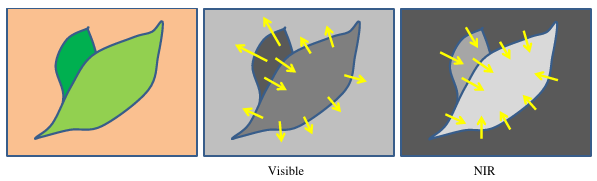
\includegraphics[width=0.6\linewidth]{../figures/contrast-inversion.png}
		\caption{
			Gradient orientation in spectral band \cite{rabatel:hal-01684135},
			we can see that the orientation of the gradient is not the same depending to the spectral band,
			making the absolute derivative an important step for matching between different spectral band.
		}
		\label{fig:vegetable-gradient}
	\end{figure}
	
	\par The affine correction attempts to help the feature matching by adding properties of epipolar lines (close).
	Thus, the matching of extracted features can be spatially bounded,
	(i) we know that the maximum translation is limited to a distance of a few pixels (less than $10$px),
	and (ii) the angle between the initial element and the matched one is limited to $[-1,1]$ degree.
	
	\paragraph{Computing the gradient} \label{sec:pre-processing} To compute the gradient of the image with a minimal impact of the light distribution (shadow, reflectance, specular, ...),
	each spectral band is normalized using Gaussian blur \cite{sage0303}, the kernel size is defined by $\floor{\ceil{image\_width^{0.4}}/2} * 2 +1$ (19 in our case)
	and the final normalized images are defined by $I/(G+1)*255$ where $I$ is the spectral band and $G$ is the Gaussian blur of those spectral bands.
	This first step minimizes the impact of the noise on the gradient and smooths the signal in case of high reflectance.
	Using this normalized image, the gradient $I_{grad}(x,y)$ is computed with the sum of absolute Sharr filter \cite{Seitz}
	for horizontal $S_x$ and vertical $S_y$ derivative, noted $I_{grad}(x,y)=\frac{1}{2}|S_x|+\frac{1}{2}|S_y|$.
	%Different types of edge detection such as Sobel, Laplacan and Canny were tested unsuccessfully (without sufficient number of matches), those not included in this study.
	Finally, all gradients $I_{grad}(x,y)$ are normalized using CLAHE \cite{zuiderveld1994contrast} to locally improve their intensity and increase the number of key points detected.% (especially for 850nm).
	%\begin{figure}[!htb]
	%	\centering
	%	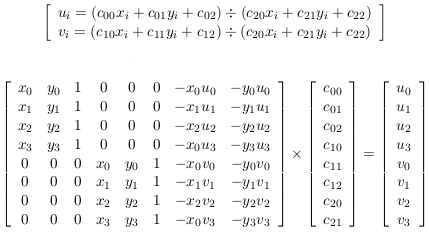
\includegraphics[width=0.6\linewidth]{../figures/math-perspective-correction.png}
	%	\caption{equation of the perspective correction}
	%	\label{eq:perspective}
	%\end{figure}
	
	\paragraph{Key-points Extractor}
	
	A key point is a point of interest. It defines what is important and distinctive in an image.
	Different types of key point extractors were available and the following more popular were tested :
	(ORB) Oriented FAST and Rotated BRIEF \cite{Rublee:2011:OEA:2355573.2356268}, 
	(AKAZE) Fast explicit diffusion for accelerated features in nonlinear scale spaces \cite{alcantarilla2011fast}, 
	(KAZE) A novel multi-scale 2D feature detection and description algorithm in nonlinear scale spaces \cite{rs10050756}, 
	(BRISK) Binary robust invariant scalable key-points \cite{leutenegger2011brisk}, 
	(AGAST) Adaptive and generic corner detection based on the accelerated segment test \cite{mair2010adaptive}, 
	(MSER) maximally stable extremal regions \cite{donoser2006efficient}, 
	(SURF) Speed-Up Robust Features \cite{bay2006surf}, 
	(FAST) FAST Algorithm for Corner Detection \cite{trajkovic1998fast}
	and (GFTT) Good Features to Track \cite{shi1994good}.
	These algorithms were largely summarized across multiple studies \cite{DantasDiasJunior, Tareen2018ACA, Zhang2016EXTENSIONAE, ali2016comparison},
	they are all available and easily usable in OpenCV, thus we have studied them by varying the most influential parameters for each of them with three modalities,
	the table \ref{tab:used-algorithms} in appendix shows all modalities and methods.
	All the results can be found in ``figures/*''.
	
	\paragraph{Key-point detection} \label{sec:perspective}
	We use one of the key-point extractors mentioned above between each spectral band gradients (all extractors are evaluated).
	For each detected key-point, we extract a descriptor using ORB features.
	We match all detected key-points to a reference spectral band (all bands are evaluated).
	All matches are filtered by distance, position and angle, to eliminate false positives along the epipolar line.
	Finally we use the function \textit{findHomography} between the key points detected/filtered with RANSAC \cite{Fischler:1981:RSC:358669.358692},
	to determine the best subset of matches to calculate the perspective correction.
	
	%\begin{figure}[!htb]
	%	\centering
	%	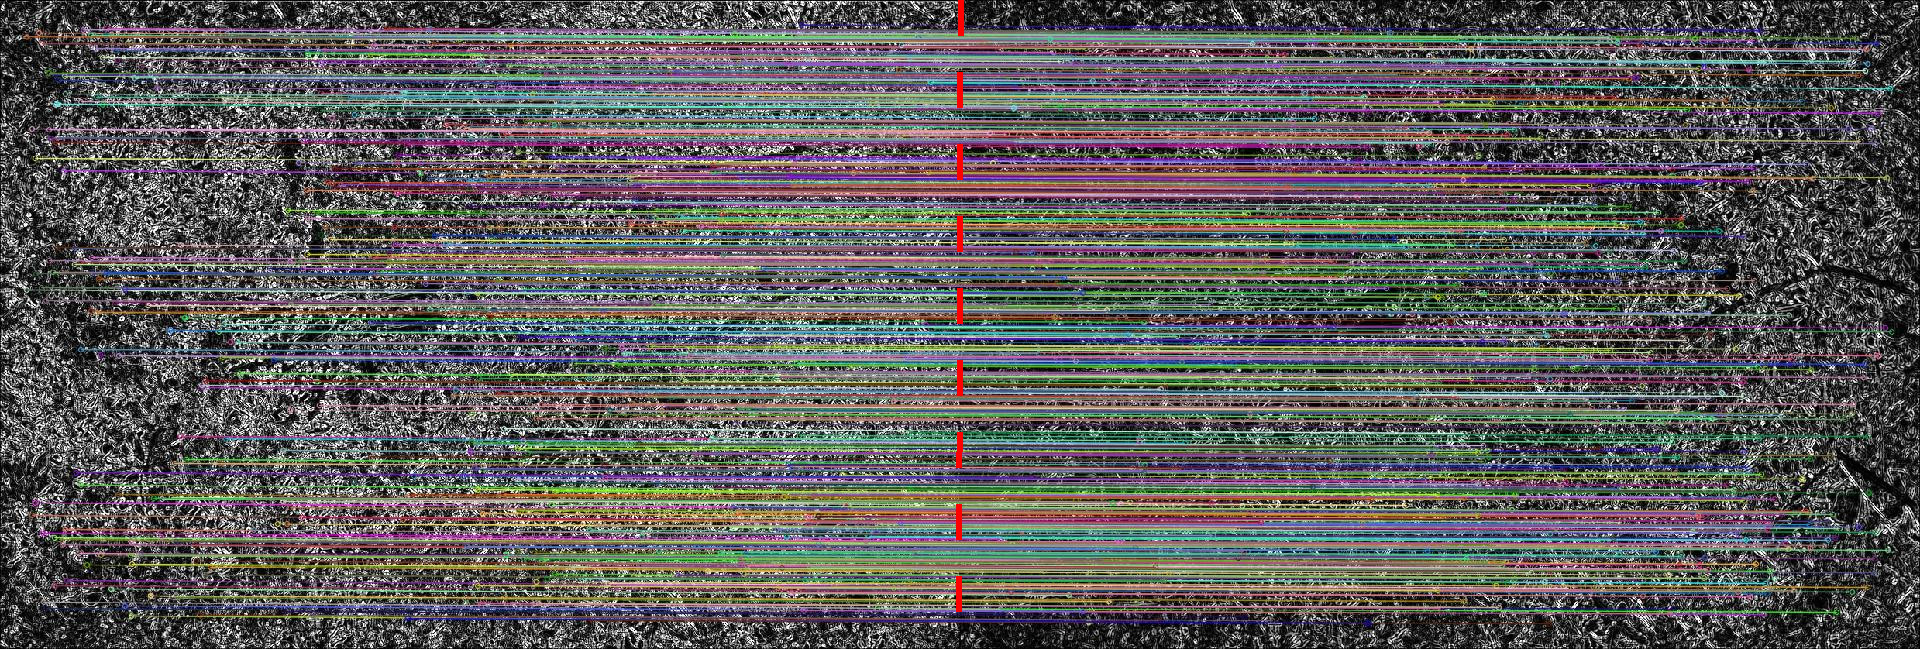
\includegraphics[width=0.7\linewidth]{../figures/prespective-feature-matching.jpg}
	%	\caption{feature matching}
	%	\label{fig:feature-matching}
	%\end{figure}
	
	\paragraph{Correction}
	
	The perspective correction between each spectral band to the reference is estimated and applied.
	Finally, all spectral bands are cropped to the minimum bounding box,
	the minimum and maximum points are obtained by applying a perspective transformation to each corner of the image.
	
	%\subsection{Re-estimating the reel height}
	%The same procedure about curve fitting \cite{More78} can be used to evaluate the inverse model between height and translation.
	%By adding the affine translation and the perspective transform of the central image point $x,y$,
	%the ``real'' translation can be evaluate. Using this value as input of the inverse model,
	%we can estimate the real height of the acquisition.
	%
	%\noindent
	%\colorbox{green}{estimating the height of each spectral bands corner} \\
	%\colorbox{green}{to the reference can enable to build the ground plan ?} \\
	%\colorbox{green}{and enable to correct the row gradient ?}
	
	\section{Results and discussion}
	
	Firstly the results will focus on affine corrections and then on the effects of the perspective correction.
	Figure \ref{fig:merged-correction} shows a zoom inside unregistred image, registred image of each correction steps at $1.6m$ and the manufacturer results.
	
	\begin{figure}[H]
		\centering
		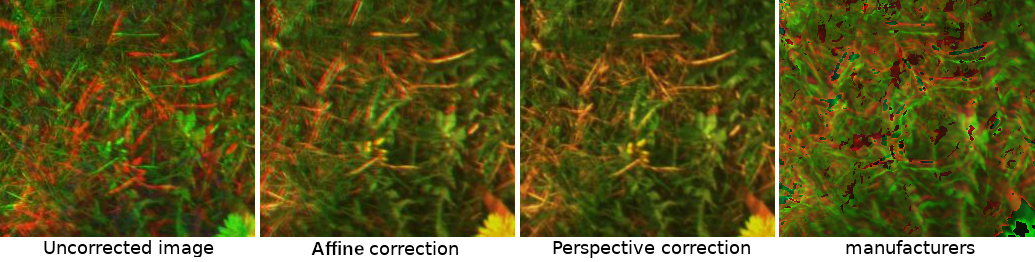
\includegraphics[width=0.7\linewidth]{../figures/merged-correction.png}
		\caption{Example of each correction and the manufacturers results}
		\label{fig:merged-correction}
	\end{figure}
	
	\subsection{Affine correction}
	
	The 6 coefficients ($A,B,C,D,X,Y$) of the affine matrix were studied according to the height of the camera in order to see their stability.
	It appears that the translation part ($X,Y$), depends on the distance of the field (appendix figure \ref{fig:affine-translation-height}).
	On this part the linear model is used to estimate the affine correction from an approximated height.
	%Due to the hard correlation between spectral bands these registration, especially between 450nm and 710-850nm (unless using normalized gradient)
	%have not been investigated and suggest that the reader should see the specific article \cite{rabatel:hal-01684135}.
	
	\begin{figure}[H]
		\centering
		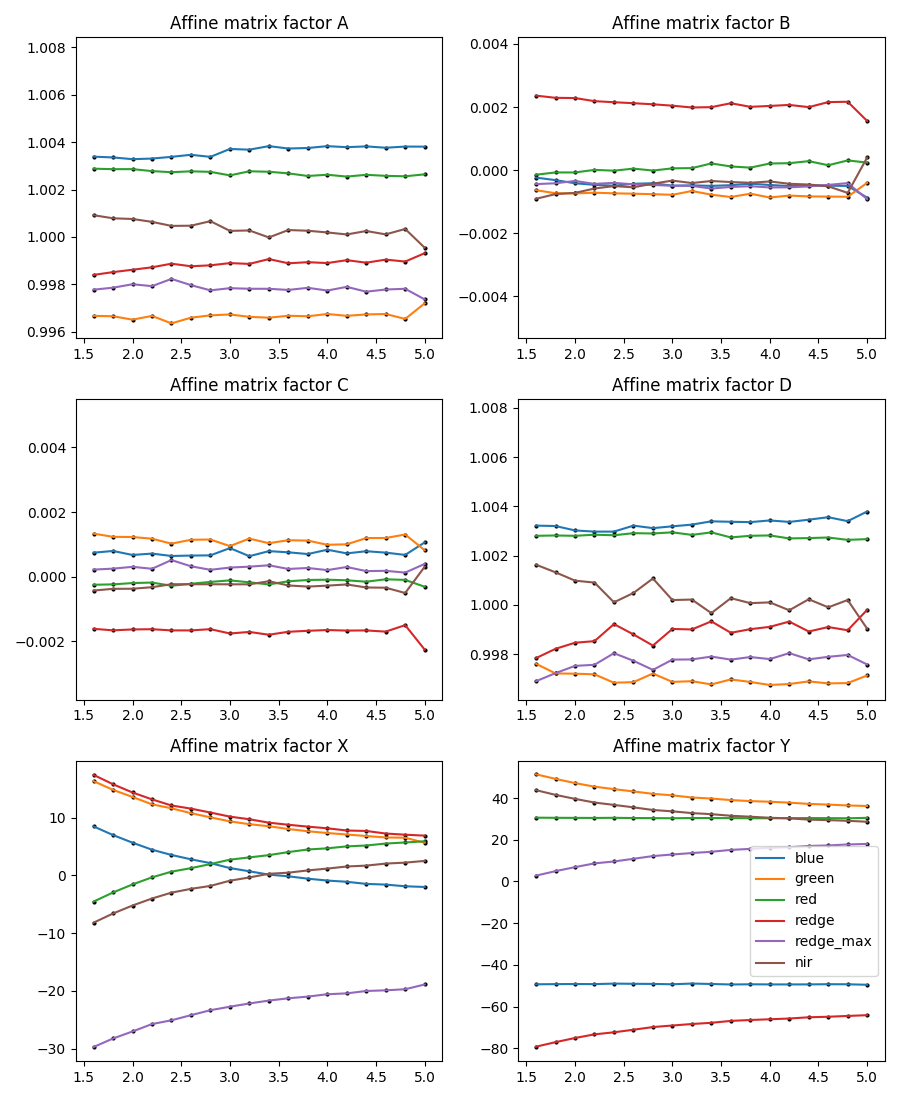
\includegraphics[width=0.5\linewidth]{../figures/affine-translation-height.png}
		\caption{Affine matrix value by height}
		\label{fig:affine-translation-height}
	\end{figure}

	Rotation and scale do not depend on the ground distance (figure \ref{fig:affine-rotation-height}).
	These factors ($A,B,C,D$) are quite stable and close to identity, as expected (accuracy depends on the spatial resolution of the board).
	As result, single calibration can be used for this part of the matrix, and the most accurate are used.
	
	\begin{figure}[H]
		\centering
		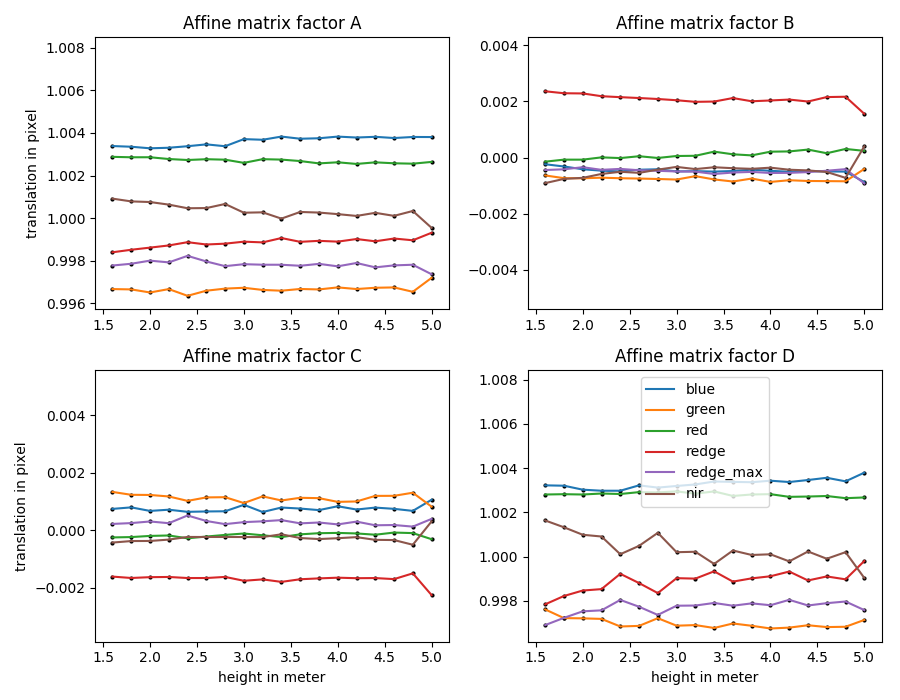
\includegraphics[width=0.5\linewidth]{../figures/affine-rotation-height.png}
		\caption{Affine matrix value by height}
		\label{fig:affine-rotation-height}
	\end{figure}
	
	%After the correction, i.e. the Affine transformation using the linear model from the approximate height,
	The remaining distance between each spectral band varies according to the distance between the real height and the nearest selected.
	These residual distances can be seen in the figure \ref{fig:affine-error},
	remember that a bias of +/- $10cm$ was set, implying superior error.
	
	\begin{figure}[H]
	\centering
		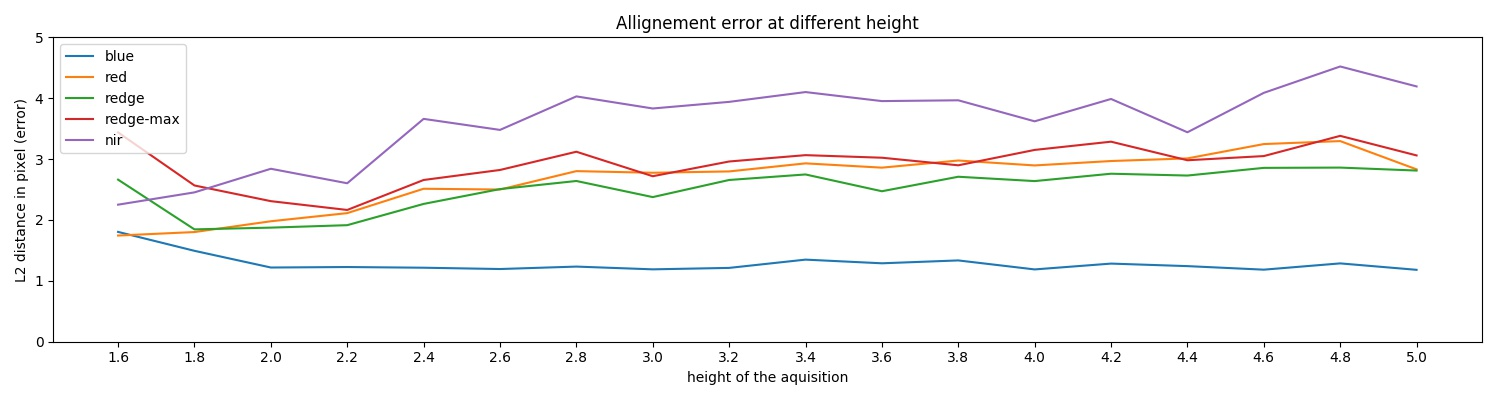
\includegraphics[width=0.8\linewidth]{../figures/affine-allignement-rmse.jpg}
		\caption{The mean distance of detected key-point before perspective correction with 570nm as spectral reference}
		\label{fig:affine-error}
	\end{figure}
	
	% https://www.lfd.uci.edu/~gohlke/code/imreg.py.html
	
	\subsection{Perspective correction}
	
	The figures \ref{fig:features-performances} shows the numbers of key-points after filtering and homographic association (minimum of all matches)
	as well as the computation time and performance ratio (matches/time) for each method.
	
	\begin{figure}[H]
		\centering
		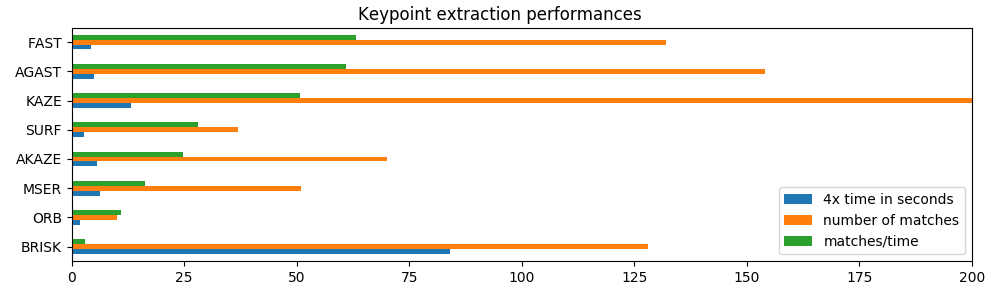
\includegraphics[width=0.9\linewidth]{../figures/comparaison-keypoint-performances.png}
		\caption{features extractor performances after filtering and homography association}
		\label{fig:features-performances}
	\end{figure}
	
	All these methods offer interesting results, the choice of method depends to the wanted balance between computation time and accuracy:
	\begin{itemize}
		\item GFTT shows the best overall performance in both computation time and number of matches
		\item FAST and AGAST1 are quite suitable too, balanced in time and with greater matches performances.
	\end{itemize}
	
	\noindent
	The other ones did not show improvement in term of time or matches:
	\begin{itemize}
		\item KAZE show correct number of matches (>200) but it's also 2.5 times slower than FAST or AGAST.
		\item AKAZE and MSER did not show benefits comparing to FAST.
		\item ORB and SURF could be excluded, the number of matches in too small to ensure the precision.
		\item BRISK shows good number of matches, at the cost of an important computation time (79 sec).
	\end{itemize}
	
	\par Increasing the number of key points matched allows a slightly higher accuracy \cite{DantasDiasJunior, }.
	For example, switching from SURF (30 results) to FAST (130 results) reduces the final residual distances from ~1.2 to ~0.9 pixel but increases the calculation time from $\approx 5$ to $\approx 8$ seconds.
	\\
	\par All methods show that the best reference spectrum is $710nm$, with the exception of SURF and GFTT which is $570nm$.
	The figure \ref{fig:features-GFTT-performances} shows the minimum number of matches between each reference spectrum and all others using the GFTT algorithm.
	Choosing the right spectral reference is important, as we can see, no correspondence is found in some cases between $650-850nm$,
	but correspondences are found between $675-710nm$ and $710-850nm$, making the $710nm$ more appropriate,
	the same behavior can be observed for the other bands and $570nm$.
	This is visible on the "all\_min" coluns, $570nm$ and $710nm$ have the best minimum number of matches.
	Other best spectral reference are available in supplementary material.
	
	\begin{figure}[H]
		\centering
		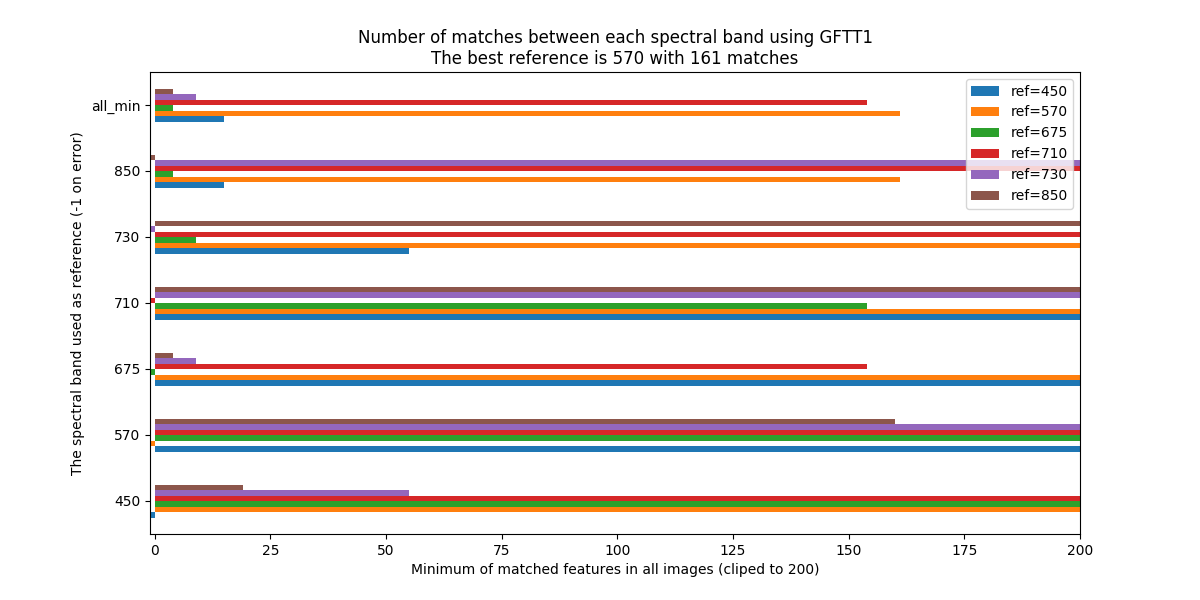
\includegraphics[width=0.9\linewidth]{../figures/comparaison-keypoint-matching-reference-GFTT1.png}
		\caption{feature GFTT performances}
		\label{fig:features-GFTT-performances}
	\end{figure}
	
	\par Residues of the perspective correction show that we have correctly registered each spectral band with a residual error of less than 1 pixel,
	the figure \ref{fig:perspective-error} shows the residual distance at different ground distances.
	
	\begin{figure}[H]
		\centering
		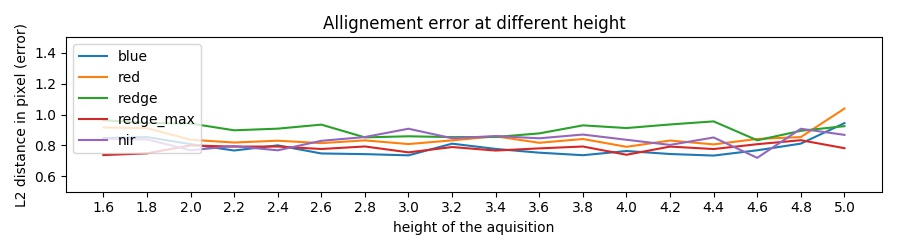
\includegraphics[width=0.8\linewidth]{../figures/prespective-allignement-rmse.jpg}
		\caption{Perspective re-projection error with GFTT1 and 570nm as reference}
		\label{fig:perspective-error}
	\end{figure}
	
	\par The figure \ref{fig:perspective-features-matching-scatter} shows the difference between detected points for two bands (red-green)
	before (left) and after (right) the perspective correction, and show that the residual errors are spatially uniform.
	
	\begin{figure}[H]
		\centering
		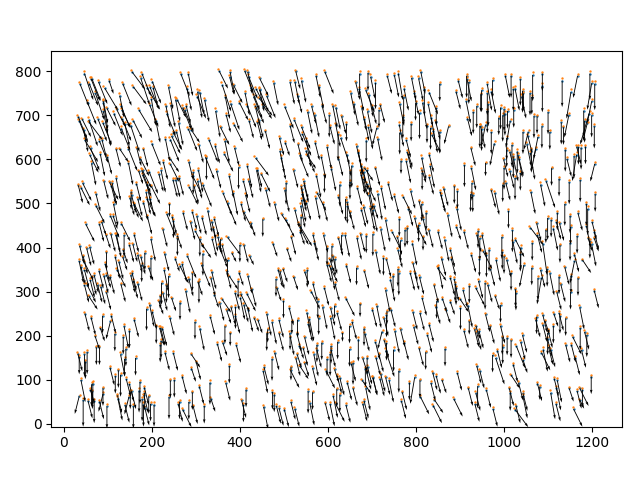
\includegraphics[width=\linewidth]{../figures/perspective-features-matching-scatter.png}
		\caption{perspective-features-matching-scatter}
		\label{fig:perspective-features-matching-scatter}
	\end{figure}
	
	\newpage
	\par The decomposition of the residual distances by angles, visible in the figure \ref{fig:residual-angle} is interesting.
	
	\begin{figure}[H]
		\centering
		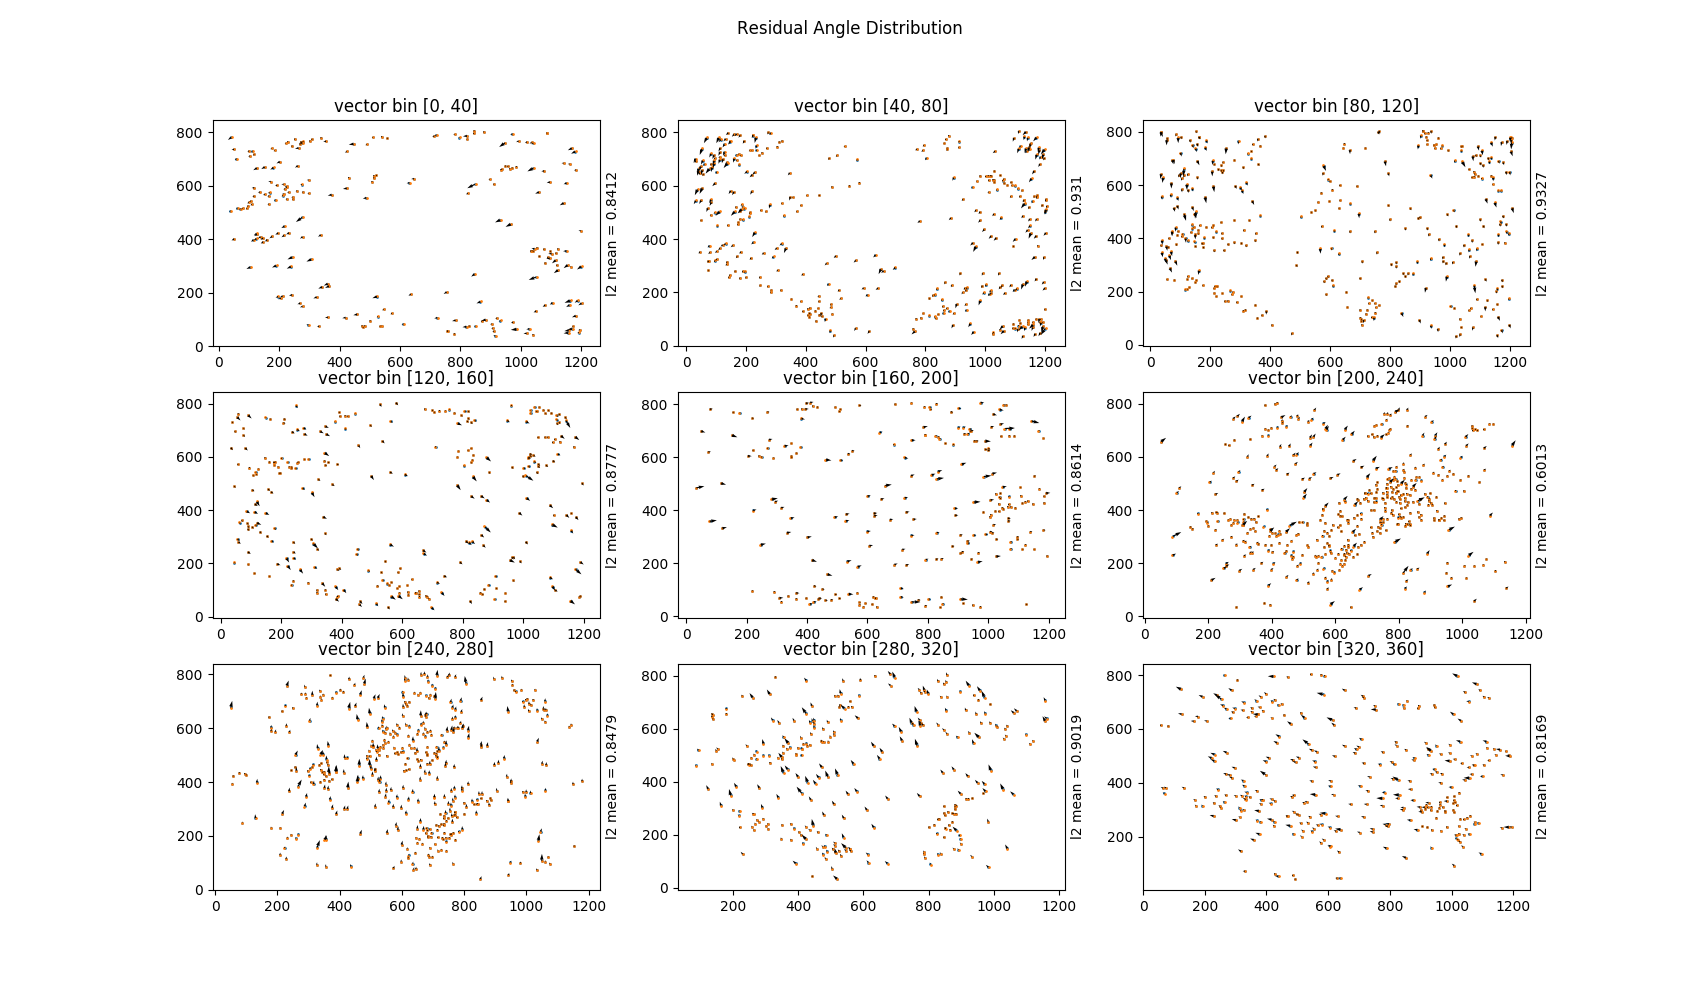
\includegraphics[width=\linewidth]{../figures/perspective-features-residual.png}
		\caption{Residual Distribution Again Angle}
		\label{fig:residual-angle}
	\end{figure}

	We can notice that the spatial distribution of the residues, for each different angle, is equally distributed.
	Our hypothesis is that the nature of the base information (spectral band + different lens) makes a small difference to the gradient break,
	which is detected by the features detector and propagated until the final correction (observed residue).
	This is interesting because these residues uniformly distributed by angle in space tend to minimize the resulting correction of its center (gradient),
	thus the detected residual error are overrated and should be less than $0.4$ pixel.

	\subsection{General discussion}
	
	\par Even if the relief of the scene is not taken into account due to the used deformation model,
	in our case, with flat ground, no difference arise.
	However, more complex deformation models \cite{Lombaert, ThinPlateSpline} can be used to improve the remaining error.
	%This type of complex deformation has not been fully evaluated, but only quickly tested through \textit{cv2.ThinPlateSplineShapeTransformer}.
	%There does not seem to be any significant improvement in most cases (with a huge computation time).
	But can also, in some cases, create large angular deformations caused by the proximity of key-points,
	of course, it's possible to filter these key-points, which also reduces the overall accuracy.
	\\
	\par Further researches can be performed on each parameter of the feature extractors, for those who need specific performance (time/precision),
	We invite anyone to download the dataset and test various combinations.
	Otherwise feature matching can be optimized, at this stage, we use brute-force matching with post filtering,
	but a different implementation that fulfill our epipolar line properties should greatly enhance the number of matches by reducing false positives.
	\\
	\par Finally, the method was tested on more than 8000 images in real conditions (not present in the study),
	randomly taken between 1.6 and 2.2 meters without registration error (always a minimum number of matches, without observed error, less than $0.9$px).
	All were acquired manually using a wheelbarrow and the camera was mounted on a pole to scan the crops along the row in the field.
	
	%%%%%%%%%%%%%%%%%%%
	
	\section{Conclusion}
	
	\par In this work, the application of different techniques for multi-spectral image registration was explored for Airphen camera.
	We have tested nine type of available OpenCV4 methods (ORB, GFTT, AGAST, FAST, AKAZE, KAZE, BRISK, SURF, MSER)
	for key-points extractors at different heights and the number of control points obtained.
	As seen in the method, the most suitable method is the GFTT (regardless of modalities 1, 2 or 3)
	with a significant number of matches and a reasonable calculation time.
	\\
	\par Furthermore, the best spectral reference was defined for each method, for example 570 for GFTT.
	We have observed a residual error of less than 1 px, supposedly caused by the difference (spectral range, lens).
	
	\section{Acknowledgments}
	
	\par The authors acknowledge support from European Union through the project H2020 IWMPRAISE \footnote{\url{https://iwmpraise.eu/}}
	(Integrated Weed Management: PRActical Implementation and Solutions for Europe)
	and from ANR Challenge ROSE through the project ROSEAU \footnote{\url{http://challenge-rose.fr/en/projet/roseau-2/}} (RObotics SEnsorimotor loops to weed AUtonomously).
	\\
	\par We would like to thanks Jones Gawain, Combaluzier Quentin, Michon Nicolas, Savi Romain and Masson Jean-Benoit
	for the realization of the metallic gantry that help us positioning the camera at different heights.
	
	\section{Supplementary material}
	
	The additional data and source code associated with this article can be found in the online version at the following address
	\url{gitlab.com/phd-thesis-adventice/phd-airphen-alignment} the access is limited,
	and we invite you to send an email to the author for full access.
	
	\section{Appendix}

	\begin{table}[H]
	\begin{tabular}{|l|c|c|c| } 
		\hline
		ABRV & 1 & 2 & 3 \\
		\hline
		ORB & nfeatures=5000 & nfeatures=10000 & nfeatures=15000 \\
		GFTT & maxCorners=5000 & maxCorners=10000 & maxCorners=15000 \\
		AGAST & threshold=71 & threshold=92 & threshold=163 \\
		FAST & threshold=71 & threshold=92 & threshold=163 \\
		AKAZE & nOctaves=1, nOctaveLayers=1 & nOctaves=2, nOctaveLayers=1 & nOctaves=2, nOctaveLayers=2 \\
		KAZE & nOctaves=4, nOctaveLayers=2 & nOctaves=4, nOctaveLayers=4 & nOctaves=2, nOctaveLayers=4 \\
		BRISK & nOctaves=0, patternScale=.1 & nOctaves=1, patternScale=.1 & nOctaves=2, patternScale=.1  \\
		SURF & nOctaves=1, nOctaveLayers=1 & nOctaves=2, nOctaveLayers=1 & nOctaves=2, nOctaveLayers=2 \\
		MSER & None & None & None \\
		\hline
	\end{tabular}
	\caption{list of algorithms with 3 variation of their parameters}
	\label{tab:used-algorithms}
	\end{table}
	
	\section{References}
	\bibliography{references.bib}
	\bibliographystyle{apalike}
	
\end{document}
